\documentclass{ximera}  


\input{../preamble.tex}



 
\title{Electrostatics Boundary Conditions} 
\author{Milica Markovic} 
\outcome{Boundary Conditions.}
\begin{document}  
\begin{abstract}  

\end{abstract}  
\maketitle    






\begin{figure}[htbp]
\begin{center}
\includegraphics[scale=0.5]{../jpg/boundaryconditions.jpg}
\end{center}
\caption{Boundary Conditions for Electric Field.}
\label{BoundaryCondition}
\end{figure}





\begin{figure}[htbp]
\begin{center}
\includegraphics[scale=0.5]{../jpg/integrationpathtangfield.jpg}
\end{center}
\caption{Integration}
\label{BoundaryCondition}
\end{figure}




\begin{figure}[htbp]
\begin{center}
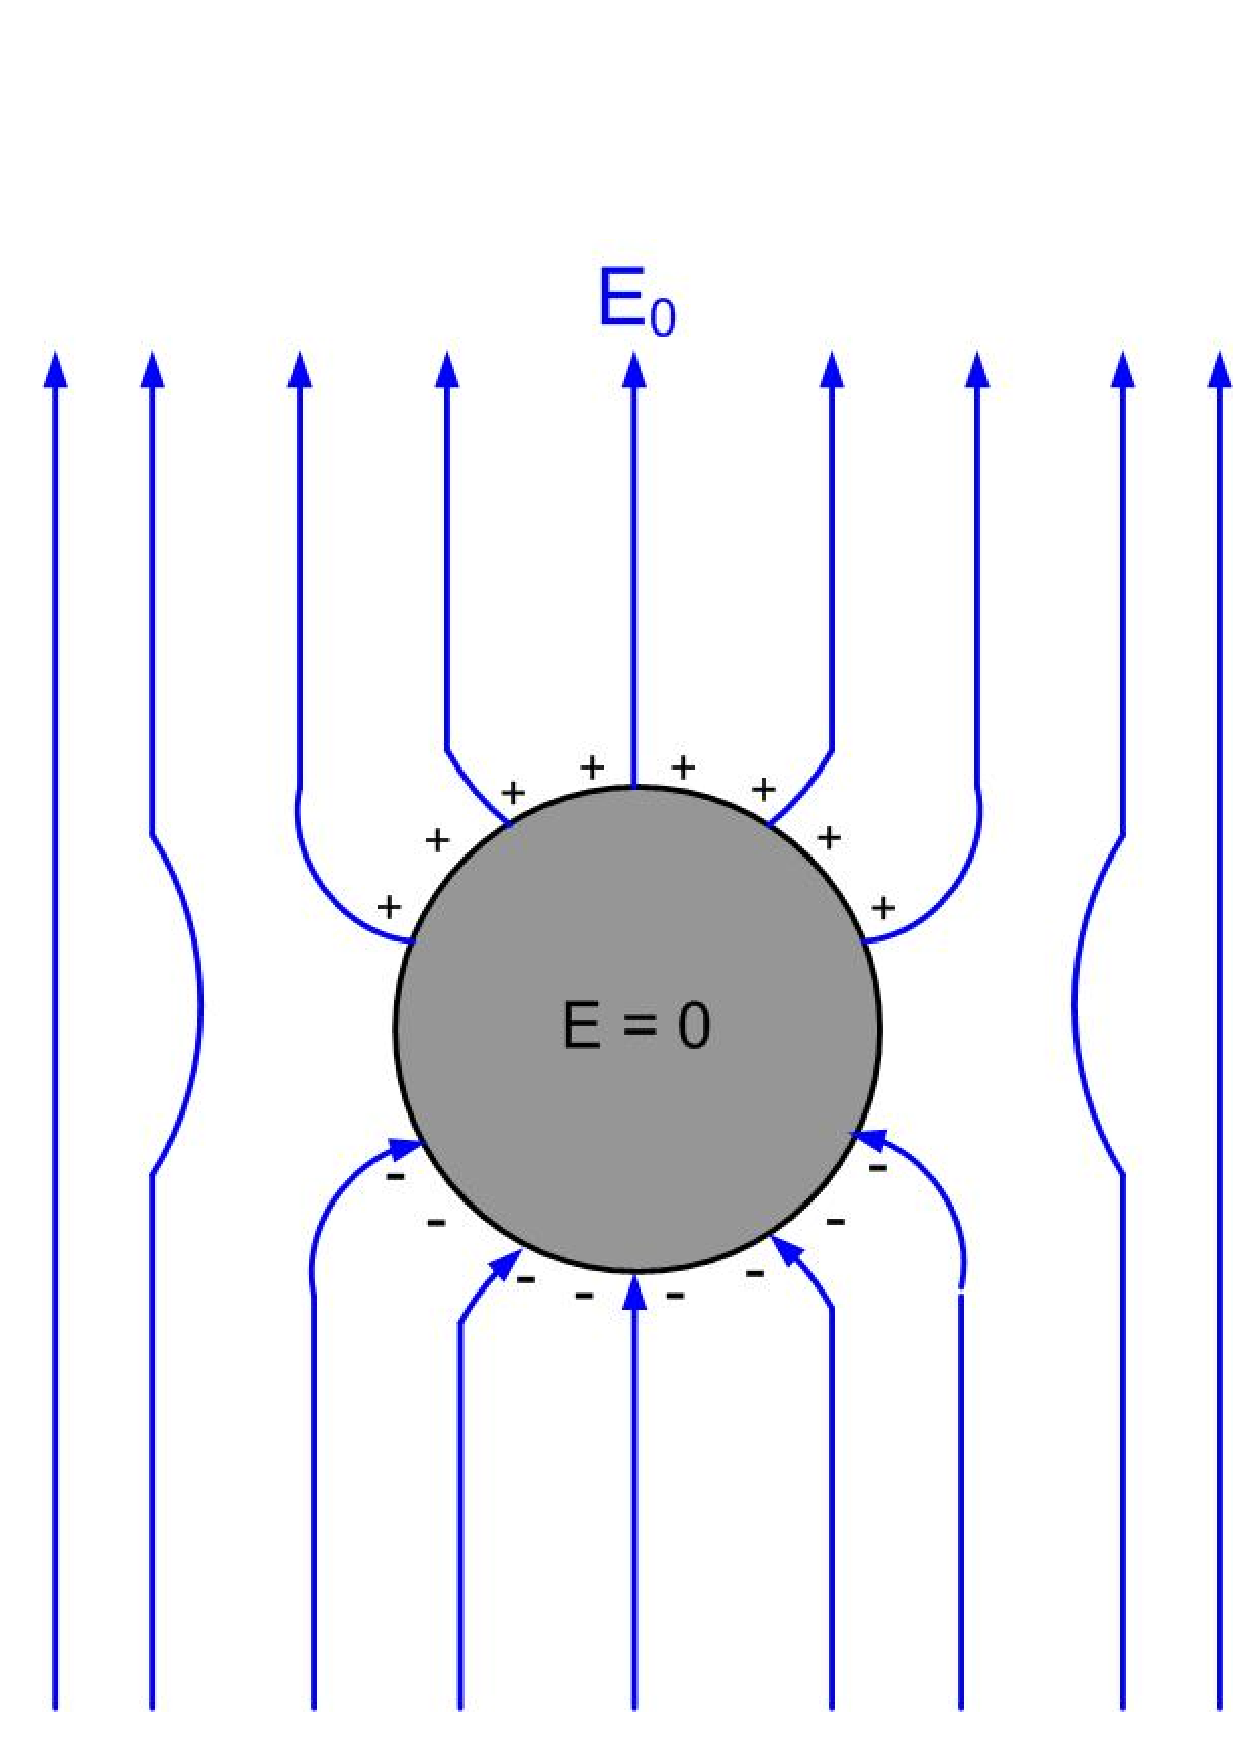
\includegraphics[scale=0.5]{../jpg/metalsphereinefield.jpg}
\end{center}
\caption{Metallic sphere in an external electric field.}
\label{BoundaryConditionMetal}
\end{figure}









\end{document} 
